\chapter{Data}\label{sec-3.data}

We conduct our empirical research using various data sources: (1) detailed transaction data provided by China’s General Administration of Customs, (2) the annual surveys from Chinese Industrial Enterprises provided by the National Bureau of Statistics of China, and (3) country-level macro data from Penn World Table 10.0. In this section, we will introduce the basic information of these datasets.

\section{Customs Transaction Records}

The first dataset we use is the transaction level records from the General Administration of Customs of China (GACC) as in \cite{manova-zhang2012}. The whole sample period ranges from 2000 to 2011. This dataset includes the most comprehensive information on all Chinese trade transactions including import and export values (denominated in US dollars), quantities, units, product names and codes, source and destination countries, and type of enterprises (e.g., state-owned, private, foreign-invested, and joint ventures), etc. Using these high-frequency trade records, we are able to compute firm–product unit values to study export or import price responses to exchange rate shocks. 

We separate the full records into export and import parts. In our analysis, each unique transaction refers to a firm-product-country-year consolidation. The categories of products in China's customs trade records are coded according to the Harmonized Coding and Description System (Harmonized System or HS) from World Customs Organization (WCO). The original data is subject to HS 8-digit classification. Since there are two major revisions of the HS system in 2002 and 2007, we aggregate HS8 product-level information to the HS6 level and then use conversion tables from the United Nations Trade Statistics to convert HS 2007 and HS 2002 codes into the older version of HS 1996 as in \cite{fan-li-yeaple2015}.

For later empirical studies, we drop unwanted observations referring to the standard of \cite{lmx2015}: (1) products with inconsistent missing information of unit or quantity; (2) special product categories such as arms (HS2=93), antiques (HS2=97), and special categories (HS2=98 and 99); (3) transactions existing for only one year without any change over time. Those outliers only make up a very small part of observations. We will refer to this sample as the "long sample" in subsequent analyses.

\section{Chinese Firm-level Data}

Our source of Chinese firm-level production and financial information is the Chinese Industrial Enterprises (CIE hereafter) database from the National Bureau of Statistics of China (NBSC). This database covers all state-owned enterprises and above-scale firms with annual sales of more than 5 million RMB. The dataset covers the period from 1999 to 2007. The number of firms each year ranges from about 130,000 in 1999 to 300,000 in 2007. The data provide details about firms’ identification code, ownership, industry type, and about 80 other variables in the balance sheet. The company information variables we use in this project include the number of employees, total wage payments, the value of fixed assets, sales income, total operation inputs, etc.

To merge this firm-level survey data with customs records, we follow the standard procedure to match the identification codes based on the contact information of firms as in \cite{fan-li-yeaple2015}. Manufacturing firms participating in international trade in the matched sample are uniquely identified by the FRDM codes and year. We drop unsatisfactory observations following the criteria of \cite{bkl2021}. This merged sample contains the overlapping time of the two datasets, i.e. from 2000 to 2007, and all indicators are in annual terms. We will refer to this combined dataset as the "matched sample" in the rest of this paper.

The summary statistics of the whole customs records, the firm information dataset, and the final matched sample are shown in panels A, B, and C in table \ref{tab3.1}, respectively.

\begin{table}[htbp]
	\centering
	\caption{Summary Statistics for Main Samples}
	\label{tab3.1}
	\resizebox{1.1\textwidth}{!}{
	\begin{threeparttable}
	\begin{tabular}{lcccccc}
		\toprule
		& \multicolumn{1}{l}{\#observations} & \multicolumn{1}{l}{Mean} & \multicolumn{1}{l}{Median} & \multicolumn{1}{l}{Std. dev} & \multicolumn{1}{l}{P10} & \multicolumn{1}{l}{P90} \\
		\textbf{Panel A: Customs records} &       &       &       &       &       &  \\
		Export Value (USD) & 18,581,221 & 424868 & 21692 & 1.04E+07 & 888   & 423436 \\
		Export Price (RMB) & 18,581,221 & 22007.45 & 30.10417 & 2229173 & 4.564519 & 556.4724 \\
		Annual Export Price Change & 11,400,795 & 0.025908 & 0.005982 & 0.665267 & -0.50011 & 0.5709025 \\
		Import Value (USD) & 14,172,315 & 439283 & 7721  & 1.98E+07 & 214   & 292720 \\
		Import Price (RMB) & 14,172,315 & 49519.78 & 111.0406 & 1411944 & 5.159389 & 10247.12 \\
		Annual Import Price Change  & 8,580,234 & 0.023625 & -0.00207 & 1.017117 & -0.8523061 & 0.9388119 \\
		&       &       &       &       &       &  \\
		\midrule
		\textbf{Panel B: Firm information} &       &       &       &       &       &  \\
		Sales Income (thousand RMB) & 1,745,511 & 78826.33 & 17630 & 714350.5 & 5318  & 111319 \\
		Employment & 1,745,511 & 262.9454 & 108   & 964.6382 & 30    & 500 \\
		Fixed Asset (thousand RMB) & 1,745,511 & 27437.2 & 4043  & 312024.8 & 573   & 36968 \\
		Operation Input (thousand RMB) & 1,745,511 & 61682.99 & 13971 & 562923.1 & 4035  & 168810 \\
		Current wage payable (thousand RMB) & 1,745,511 & 3730.157 & 1121  & 28699.16 & 266   & 6300 \\
		&       &       &       &       &       &  \\
		\midrule
		\textbf{Panel C: Matched sample} &       &       &       &       &       &  \\
		Export Value (USD) & 3,168,876 & 880187.2 & 33693 & 4.66E+07 & 1376  & 712735 \\
		Export Price (RMB) & 3,168,876 & 18326.68 & 28.31701 & 1893237 & 4.995613 & 398.6719 \\
		Annual Export Price Change & 1,829,966 & 0.023539 & 0.006083 & 0.682097 & -0.48284 & 0.550056 \\
		Import Value (USD) & 3,280,928 & 1120261 & 11139 & 2.36E+07 & 266   & 529584 \\
		Import Price (RMB) & 3,280,928 & 29955.95 & 76.56041 & 525990.1 & 4.966081 & 5614.432 \\
		Annual Import Price Change  & 1,827,983 & -0.08694 & -0.00105 & 1.34694 & -1.20575 & 1.013989 \\
		\bottomrule
	\end{tabular}
	\begin{tablenotes}
		\footnotesize
		\item[*] This table shows the summary statistics of some important variables in our three major datasets. Panel A and panel C describe the total annual values, annual average prices, and price changes for the whole customs records and the matched sample, respectively. The observations in panel A and panel C are at the firm-product-country-year level. The trade values in panel A and panel C are in US dollars while prices are in RMB. Panel B describes sales and costs information of Chinese manufacturing firms during 2000-2007. The money values in panel B are in thousands of RMB. The observations in panel B are at the firm-year level.
	\end{tablenotes}
	\end{threeparttable}
	}
\end{table}

A notable point is that for all variables involved in the amount of money in the table, the mean is much larger than the median, and the mean of some variables is even larger than its 90\% quantile. This means that the distribution of trade value is very uneven, with a few large transactions accounting for the majority of trade volume.

\section{Country-level Macro Data}

We obtain bilateral nominal exchange rates and price level of household consumption from the newest Penn World Table (PWT 10.0) (referring to \cite{feenstra2015}). From the whole table, we keep 183 countries (or districts) using 136 different fiat currencies, which have full records of exchange rates during the period from 1999 to 2011. 

The bilateral nominal exchange rate is defined as the number of home currency units that can purchase a unit of foreign currency. An increase in $NER_{ct}$ means a nominal depreciation of the Chinese RMB against this currency from country $c$. Following LMX \cite{lmx2015}, the CPI-based real exchange rate ($RER_{ct}$) is defined as the nominal exchange rate multiplied by the foreign consumer price index (CPI) and divided by the Chinese consumer price index (CPI) at the same year, which is

$$
RER_{ct}=NER_{ct} \cdot \frac{CPI_{ct}}{CPI_{CHN,t}}.
$$

Again, an increase in $RER_{ct}$ means a real depreciation of the Chinese RMB against the foreign country's c currency. In later specifications, we mainly use the first difference of the logarithm of the real exchange rate to represent exchange rate changes.

We saw substantial variations in RMB exchange rate fluctuations against different countries including its major trading partners during the period. We could observe that the real exchange rate against the US dollar did not change a lot in 2000-2004 due to the nominal pegging scheme of RMB to US dollars. In July 2005, the peg was lifted to a slight appreciation of RMB against US dollars as a result of the evolution of exchange policy. The currency exchange rates of China's other major trading partners also fluctuated to varying degrees during this period. Changes in nominal and real exchange rates for these countries (level in 1999 as base value 100) are shown in figures \ref{fig3.1} and \ref{fig3.2}.

\begin{figure}[htbp]
	\centering
	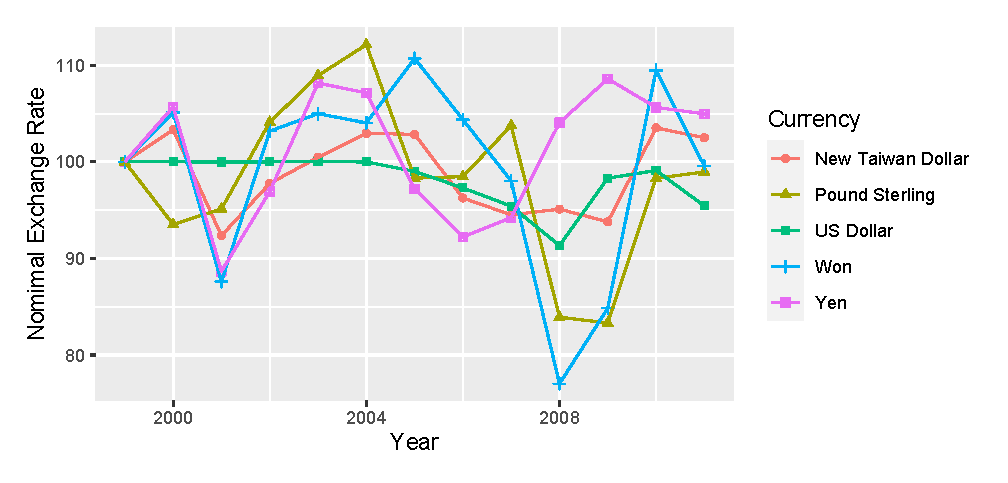
\includegraphics[width=1\textwidth]{figure/figure1.eps}
	\caption{Nominal exchange rates of China's major trading partners (1999-2011)}
	\label{fig3.1}
\end{figure}

\begin{figure}[htbp]
	\centering
	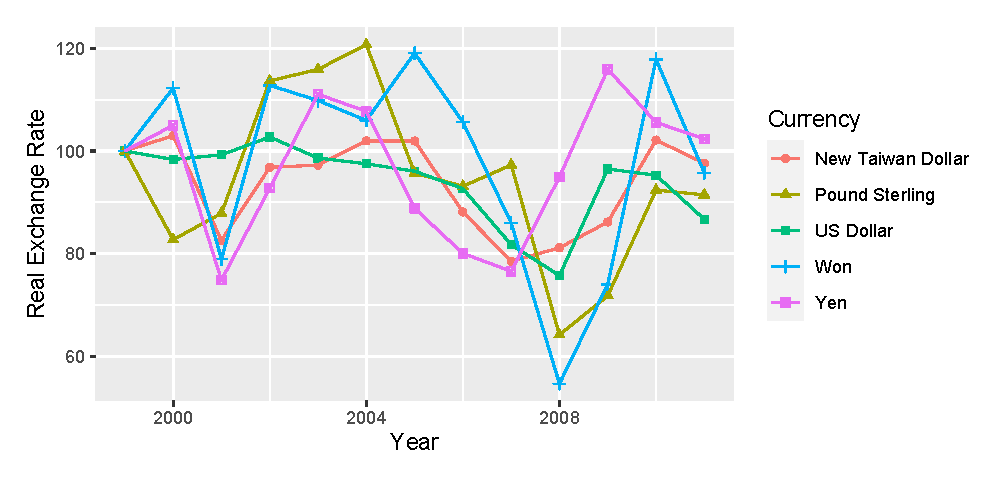
\includegraphics[width=1\textwidth]{figure/figure2.eps}
	\caption{Real exchange rates of China's major trading partners (1999-2011)}
	\label{fig3.2}
\end{figure}

In addition to nominal and real exchange rates, we also use the real GDP of the destination countries from PWT 10.0. The real GDP is computed with national-accounts growth rates. The controls of real GDP changes of the destination country, $\Delta RGDP_{ct}$, help us exclude the effect of economic growth on price movements. All macro variables including exchange rates and real GDPs are in annual terms to match the firm information survey.